\documentclass[12]{article}
\usepackage[spanish,english]{babel}
%\usepackage[spanish]{babel}
\usepackage[utf8]{inputenc}
\usepackage{graphicx}
\usepackage{epsfig}
\usepackage{multirow}
\usepackage{multicol,caption}
\usepackage{amsthm} % Theorem Formatting
\usepackage{amssymb}    % Math symbols such as \mathbb
\usepackage{color}
\usepackage{hyperref}
\usepackage[none]{hyphenat}
\usepackage{appendix}
\renewcommand{\appendixname}{Anexo}
\renewcommand{\appendixtocname}{LISTA DE ANEXOS}
\renewcommand{\appendixpagename}{Anexos}
%\renewcommand{\tablename}{Tabla}
%\def\tablename{Cuadro}% por \def\tablename{Tabla}% 
\newenvironment{Figure}
{\par\medskip\noindent\minipage{\linewidth}}
{\endminipage\par\medskip}
\addto\captionsspanish{%
\def\tablename{Tabla}%
}
\topmargin  = 10pt
\oddsidemargin  = -0.5in
%\headheight = 12pt
%\headsep    = 15pt
%\footskip   = 15pt
\textheight = 21.5 cm
\textwidth  = 18.5cm
\tolerance=10000
\title{\bf{Calculo de la longitud de onda de la radiación de un diodo led infrarrojo, utilizando el modulo motorizado infrarossi y su software de control Free infrarossi}}
\author{Julian Salamanca\footnote{jasalamanca@udistrital.edu.co}, Diego Parra\footnote{diegoestudianteud1@gmail.com} \\
  Universidad Distrital, Calle 3 No 26A-40 Bogotá-Colombia\\
  Grupo de Física e Informática ``FISINFOR''
}
\date{\today}
\begin{document}
%\def\tablename{Cuadro}% por \def \tablename{Tabla}% 
\renewcommand{\tablename}{Tabla}
\maketitle
\vspace{-0.8cm}
\selectlanguage{english}

\begin{abstract}
In this paper calculated the wavelength emitted by  an infrared LED diode using a diffraction grating, infrarossi motorized module and control software  free infrarossi; a GNU-Linux environment, highlighting the functionality of this instrument in illustrating the property of electromagnetic waves and the duality wave - corpuscle. \\
{\bf{Keywords:}} Motor module, infrared sensors, microcontroller module bluetooth, electromagnetic wave, diffraction.


\selectlanguage{spanish}
\begin{center}
{\bf{Resumen}} 
\end{center}
El presente trabajo calcula la longitud de onda emitida por un diodo led infrarrojo, utilizando una rejilla de difracción, el modulo motorizado  infrarossi y su software de control free infrarossi; en un entorno GNU-linux, resaltando la funcionalidad de este instrumento en la ilustración de la propiedad de la ondas electromagnéticas y su dualidad onda – corpúsculo. \\
{\bf{Descriptores:}} Modulo motorizado, sensores infrarrojos, microcontrolador, modulo bluetooth, ondas electromagnéticas, difracción. 
\end{abstract}

%tabla de contenido sin numeracion
%\renewcommand\contentsname{\centering TABLA DE CONTENIDO}
%\thispagestyle{empty}
%\setcounter{page}{1}
%\tableofcontents
%\clearpage

%lista de figuras
%\renewcommand\listfigurename{\centering LISTA DE FIGURAS}
%\listoffigures
%\clearpage

%lista de tablas
% \renewcommand\listtablename{\centering LISTA DE TABLAS}
% \listoftables
% \clearpage

\begin{multicols}{2}
\section{Introducción}
Los fenómenos de las ondas siempre han fascinado nuestros pensamientos y tratamos de acercarnos a estos fenómenos para tratar de entenderlos, es allí donde la física con ayuda de la matemática muestran su majestuosidad, al explicar de manera muy detallada estos fenómenos de transporte; la difracción es una de estas propiedades, la cual esta muy presente en la vida diaria y con la ayuda del modulo motorizado infrarossi y su software de control free infrarossi, se pretende ilustrar este fenómeno físico y calcular la longitud de onda propia producida por un diodo infrarrojo.\\ \\
"Un cuerpo opaco colocado a medio camino entre una pantalla y una fuente puntual proyecta una sombra complicada hecha en regiones claras y oscuras muy diferentes de las que podría esperarse de los principios básicos de la óptica geométrica. El trabajo de Franceso Grimaldi en el siglo XVII fue el primer estudio detallado que se publicó sobre esta desviación de la luz de su propagación rectilínea."\cite{OPTICA} \\ \\
"A la que denomino difracción. El efecto es una característica general de los fenómenos ondulatorios que ocurren donde quiera que una parte de un frente de onda de onda ya sea sonido, onda material o luz, esté obstruida de alguna manera. Si al encontrar un obstáculo transparente u opaco se altera la amplitud o la fase de una región del frente de onda, esto produciría difracción. Los Varios segmentos del frente de onda que se propagan más allá del obstáculo interfieren, produciendo aquella distribución de densidad de energía particular denominada figura de difracción. No hay distinción física significativa entre interferencia y difracción. Sin embargo, se ha vuelto algo común, aunque no siempre apropiado, hablar de interferencia cuando se analiza la superposición de solamente unas pocas ondas y de difracción cuando se trata de un gran número de onda."\cite{OPTICA}


\section{Marco teórico}

Una red de difracción es un conjunto repetitivo de elementos difractores de una onda emergente, bien sean aberturas u obstáculos, que tienen el efecto de producir alteraciones periódicas en la fase, amplitud o ambas. Uno de los más simples de tales conjuntos es la configuración de rendijas múltiples. Parece que fue inventado por el astrónomo americano David Rittenhouse hacia 1785. Algunos años más tarde Joseph Von Fraunhofer redescubrió, por su cuenta, este principio y siguió aportando un buen número de contribuciones importantes tanto a la teoría como a la tecnología de redes.\\ \\ 
Los primeros dispositivos eran en realidad conjuntos de rendijas múltiples, que consistían por lo general en un retículo de alambre muy fino o hilo enrollado y extendido entre dos tornillos paralelos que servían como espaciadores. Al pasar a través de semejante sistema, un frente de onda se encuentra con regiones opacas y transparentes alternadas, sufriendo una modulación en amplitud. Así mismo, una configuración múltiple de rendijas se denomina red de transmisión de amplitud. Otra forma más corriente de red de transmisión se hace rayando o raspando  unas hendiduras paralelas en la superficie de una lámina de cristal clara y plana. Cada raspadura sirve como fuente de luz esparcida, formando juntas un conjunto regular de fuentes lineales paralelas. Cuando la red es totalmente transparente, de tal manera que la modulación en amplitud sea despreciable, las variaciones regulares del espesor óptico a través del retículo dan una modulación en fase y tenemos lo que se denomina red de transmisión de fase. En la representación de Huygens -Fresnel podemos visualizar los trenes de onda como radiados con diferentes fases sobre la superficie de la red. Un frente de onda emergente contiene, por consiguiente, unas variaciones periódicas en su forma más que en su amplitud lo cual, a su vez, equivale a una distribución angular de las ondas constitutivas. \\ \\
Al reflejarse en esta clase de red, la luz esparcida por las varias caracteristicas periodicas de la superficie llegaran a un punto P con una relación de fase definida. El patrón de interferencia correspondiente engendrado despues de la reflexión es muy similar al que se produce por transmisión. Las redes diseñadas especificamente para funcionarde esta manera se denomina redes de reflexión de fase. Tradicionalmente, las redes de esta clase son rayadas sobre películas finas de aluminio que han sido evaporadas sobre bloques de vidrio ópticamente planos. Puesto que el aluminio es bastante blando, hay menos desgaste de la herramienta de rayar de diamante, siendo tambien mejor reflector en la región ultravioleta. \\ \\
Si miramos perpendicularmente a través de una red de transmisión hacia una fuente lineal paralela distante, los ojos servirían como lente de enfoque para la distribución de difracción.
La ecuación que describe el fenomeno fisico se denomina ecuación de red para incidencia normal. 
\begin{equation}
a*sin(\theta _m)= m\lambda 
\end{equation}

Los valores valores de de m especifican el orden de diversos máximos principales. Para una fuente que tenga un espectro continuo ancho, tal como un filamento de tungsteno, la imagen de orden cero, $ m = 0 $, corresponde a la imagen blanca de la fuente no desviada $ \theta _0 = 0 $. La ecuación de red depende de $\lambda$ y así, y así para cualquier valor de m $\ne = 0$, las distintas imágenes coloreadas de la fuente correspondientes a ángulos ligeramente diferentes $(\theta _m)$, se dispersa en un espectro continuo. Las regiones ocupadas por los débiles máximos secundarios aparecerán como bandas aparentemente desprovistas de luz. El espectro de primer orden $m = \frac{+}{-}1$ aparece a cada lado de $\theta = 0$ y es seguido, junto con intervalos alternados de oscuridad, por los espectros de orden superior, $m = \frac{+}{-}1, \frac{+}{-}2$, etc. Obsérvese que entre más pequeño sea el valor de a en la ecuación 1, menor será el número de órdenes visibles. 
\
\section{Montaje experimental}
\subsection{Materiales del montaje}
Para la realización de este montaje se utilizarón los siguientes materiales:
\begin{enumerate}
\item[a.] Ordenador con sistema operativo GNU-Linux.
\item[b.] Modulo motorizado infrarossi.
\item[c.] Software de control free infrarossi.
\item[d.] Fuente emisora de fotones infrarrojos.
\item[e.] Modulo bluetooth para pc.
\item[f.] Rejilla de difracción de 670 lineas por milimetro 
\end{enumerate}

\subsection{Montaje}
Colocar la fuente emisora de fotones infrarrojos y frente a ella la rejilla de difracción, luego colocar el modulo motorizado infrarossi a 40 cm de la fuente emisora, como se muestra en la figura 1. \\ \\

Abrir una terminal de GNU-Linux y escribir en el, infrarossi oprimir enter y la clave de superusuario, luego de abrir el programa debe oprimir el boton on, esperar que se empareje el bluetooth, una vez emparejado el bluetooth el programa desplegara un tercer menú, oprimir el botón de difracción y esperar que el programa tome los datos necesarios.
\begin{Figure}	
\center
\begin{tabular}{|l|r|}
\hline
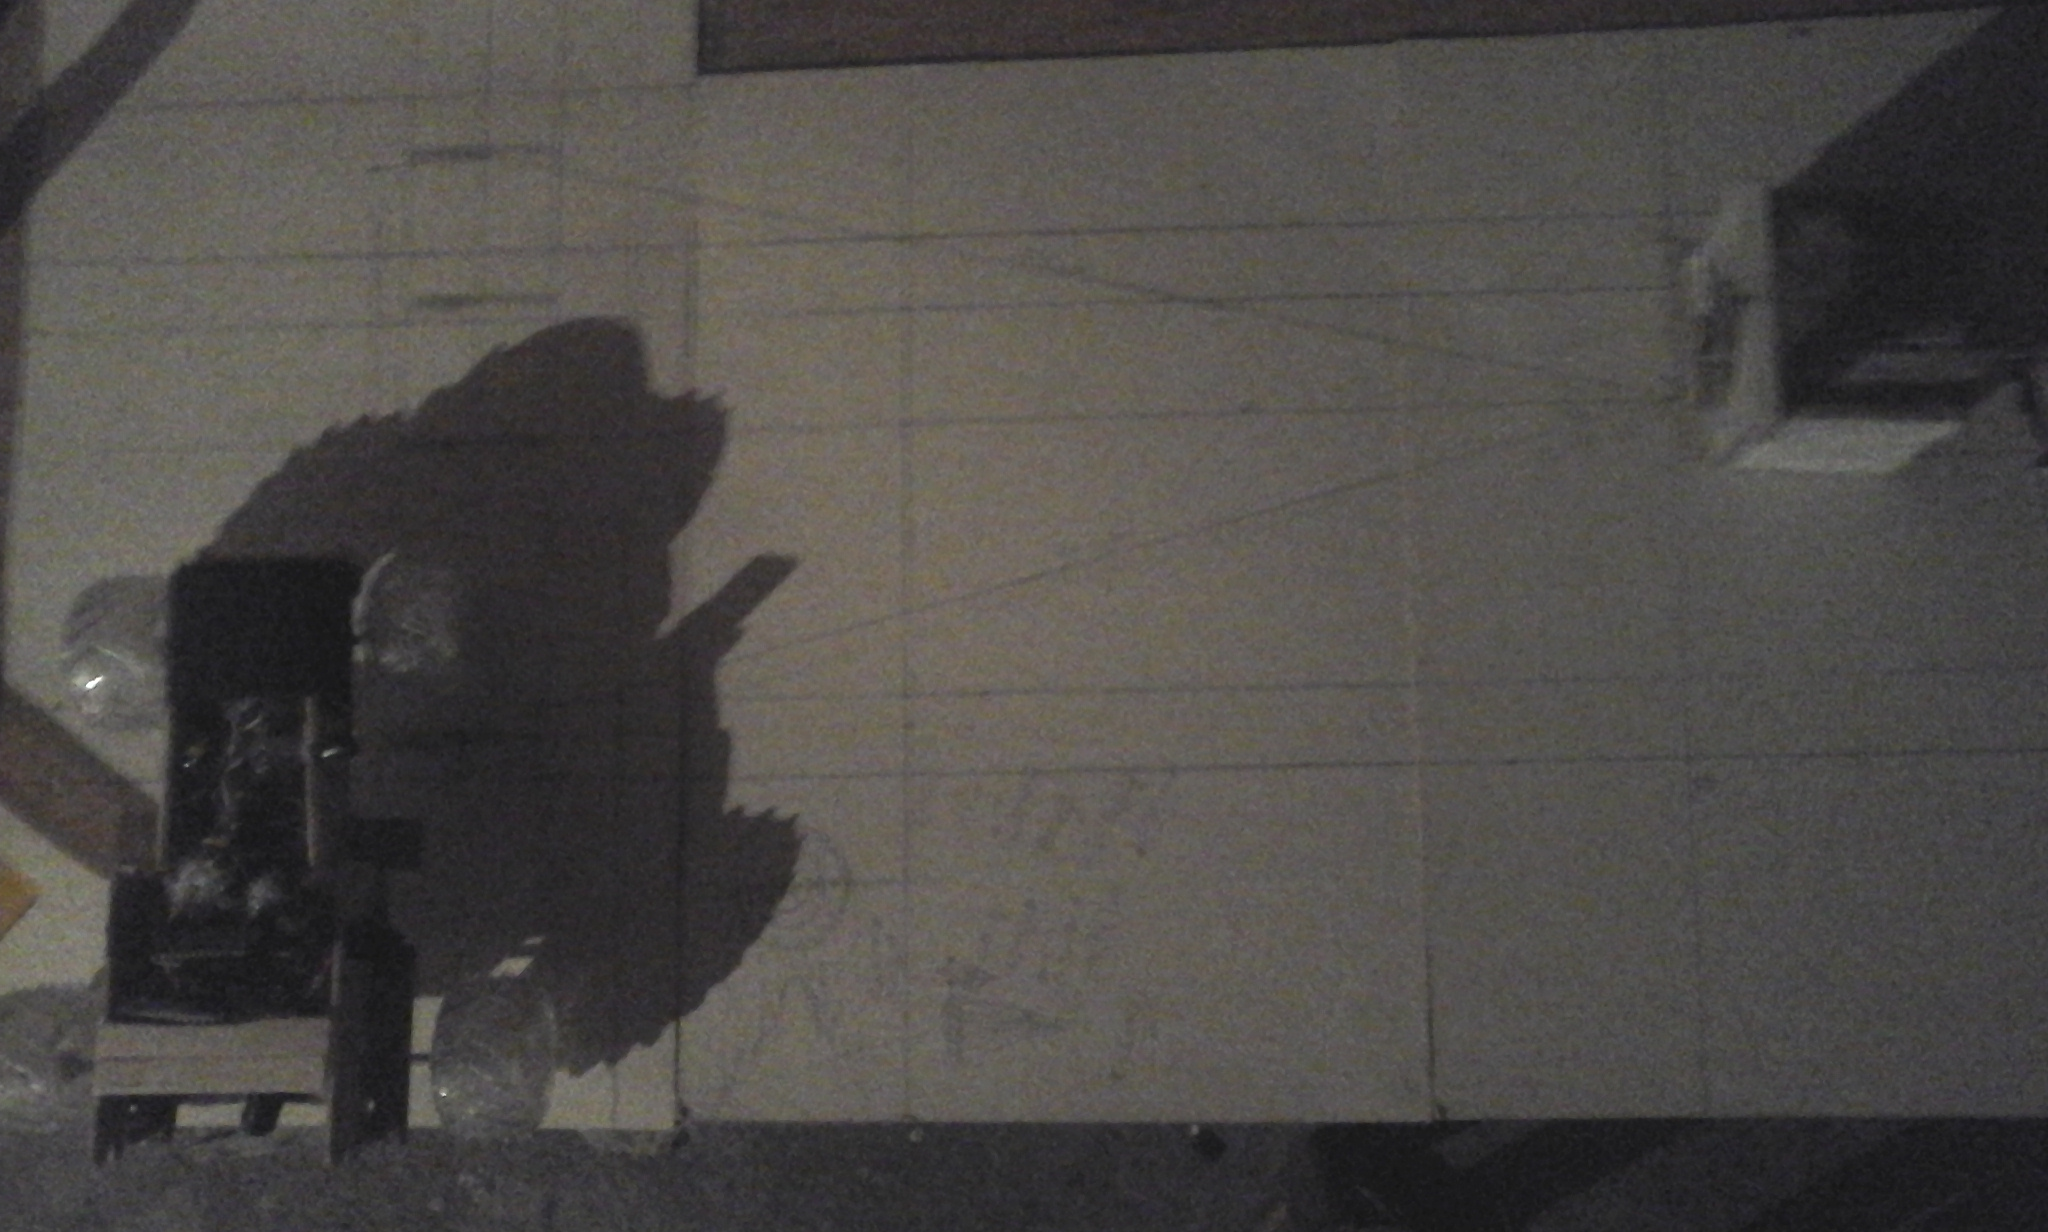
\includegraphics[width=8cm, height=6cm]{img/mon_difraccion.png} \\ \hline
\end{tabular}
\captionof{figure}{Imagen del montaje para la difracción utilizando el modulo motorizado infrarossi.}
\label{fig:g1}
\end{Figure}

\section{Análisis de resultados}
El programa free infrarossi después de terminar de recoger los datos realiza un análisis estadístico de los mismos y en una ventana aparte realiza la gráfica de los datos y predice la longitud de onda del diodo con una exactitud de $\frac{+}{-} 71 nm$
\begin{Figure}	
\center
\begin{tabular}{|l|r|}
\hline
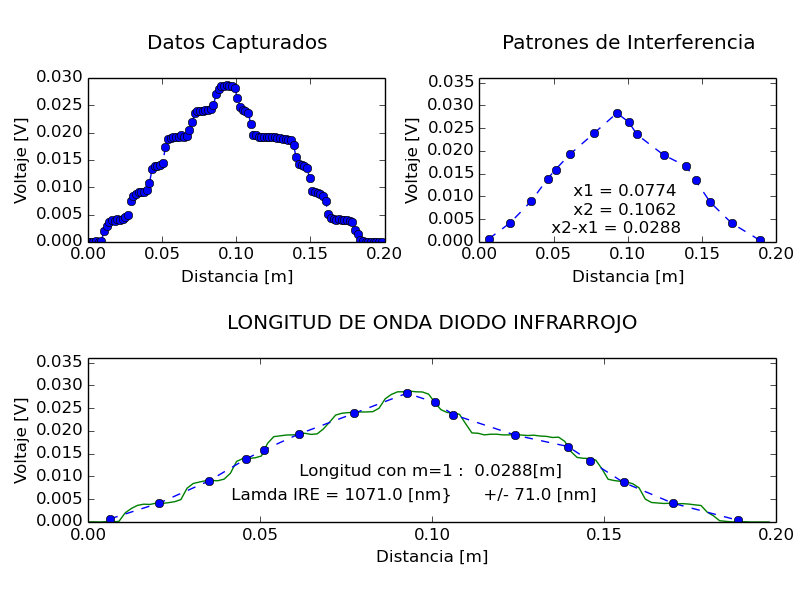
\includegraphics[width=8cm, height=6cm]{img/Graficas.png} \\ \hline
\end{tabular}
\captionof{figure}{Imagen generada por el programa free infrarossi.}
\label{fig:g1}
\end{Figure}

\section{Conclusiones}
El modulo motorizado infrarossi y su software de control free infrarossi,  es una herramienta muy potente al momento de ilustrar la propiedad de difracción de las ondas electromagneticas.
EL software de control free infrarossi es muy potente pues permite tener un margen de error de $\frac{+}{-}71 nm$, lo cual es 

\begin{thebibliography}{99}

\bibitem{OPTICA} Hecht, E., Dal Col, R., Talavera, R. W., \& Pérez, J. M. G. (2000). Óptica. Addison Wesley.
\end{thebibliography}
\end{multicols}

\end{document}

